\section{Results}

\subsection{Bias-variance ratio}

We calculated $\biasvarratio$ on the test data, shown in
Tab.~\ref{tab:summarise_new_data}. An
uncertainty on $\biasvarratio$ by performing a bootstrap sample
\cite{efron1994introduction},
where we randomly sample from both fits and replicas and re-calculate
$\biasvarratio$, the value and error presented in the table is then the mean
and standard deviation across bootstrap samples. We checked that the distribution
of the estimator across bootstrap samples is indeed Gaussian. We also checked
that increasing the number of fits and replicas reduced the bootstrap error but
the central values were the same within the estimated bootstrap uncertainities.

\begin{table}[hb]
    \begin{center}
        \begin{tabular}{lr}
            \toprule
            {}     &  $\biasvarratio$ \\
            \midrule
            Total  &  $1.03\pm0.05$   \\
            \bottomrule
            \end{tabular}
    \end{center}
    \caption{
        The bias-variance ratio, $\biasvarratio$, for unseen data, summarised in
        Tab.~\ref{tab:summarise_new_data}. The uncertainty is estimated by
        performing a bootstrap sample across fits and replicas and calculating
        the standard deviation. We see that overall $\biasvarratio$ is consistent
        with 1, within uncertainities. This gives a good indication that, at least
        for the unseen data used in this study, the uncertainities are faithful.
    }
    \label{tab:biasvarratio}
\end{table}

One can also compare qualitatively the distribution of bias across fits, to the
distribution of the difference between replica predictions and expectation
values of predictions (in units of the covariance) across different fits
and replicas. The square root ratio of the mean of these two distributions
is precisely $\biasvarratio$.

\begin{figure}[ht]
    \centering
    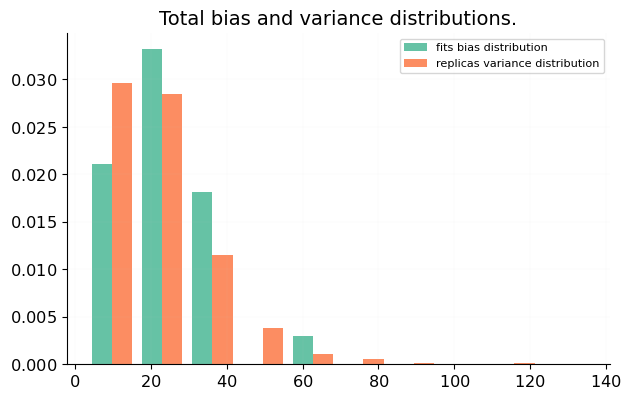
\includegraphics[width=0.8 \textwidth]{plot_bias_variance_distributions_total.png}
    \caption{The green histogram is the distribution of the total bias across fits,
    the orange histogram is the distribution of the difference between the
    replica and central predictions squared, in units of the covariance
    across all fits and replicas. This gives a qualitative picture of the full
    distribution, in Tab.~\ref{tab:biasvarratio} we compare the square root of the
    mean of each distribution.}
\end{figure}

\subsection{Comparison to quantile statistics}

As discussed in Sec.~\ref{sec:QuantileStatistics}, one can define an analogous
estimator in data space, based upon $\xi_{n\sigma}$, which was defined on a grid
of points in $x$ and $Q^2$ in PDF space in \cite{nnpdf30}. There is not
a one-to-one correspondence
between this and $\biasvarratio$, but a loose approximation using
Eq.~\ref{eq:expectedxi}. In Tab.~\ref{tab:xicomparison} we compare the estimated
$\xi_{1\sigma}$ from
subsituting $\biasvarratio$ into Eq.~\ref{eq:expectedxi} and to the
measured value.

\begin{table}[hb]
    \begin{center}
        \begin{tabular}{lrr}
            \toprule
            {}     & $\xi_{1\sigma}$ & $\erf(\biasvarratio/\sqrt{2})$ \\
            \midrule
            Total  & $0.69\pm0.02$   & $0.67\pm0.03$                  \\
            \bottomrule
            \end{tabular}
    \end{center}
    \caption{
        Comparing the measured value of $\xi_1\sigma$ and the estimated
        value from $\biasvarratio$. The two values are consistent, which
        suggests the approximation that the ratio of uncertainties is
        approximately the same across all data is not completely invalidated.
        Not only are the measured value and estimated value from $\biasvarratio$
        self consistent, but they are also consistent with $0.68$, which
        further supports the argument that the model uncertainities are
        faithful.
    }
    \label{tab:xicomparison}
\end{table}

Despite the assumptions entering each of the two estimators differing, we see
good agreement between the $\xi_{1\sigma}$ estimated from $\biasvarratio$
and that measured directly. We find this result reassuring, since it indicates
not only that the total uncertainty averaged across all data is faithful, but
also that the uncertainty on each data point seems faithful. If the results
differed it would indicate some kind of imbalance, where some components
of the uncertainty are correctly represented by the replicas but other directions
are not.
